În ziua de astăzi, rețele de socializare au devenit foarte populare în rândul utilizatorilor 
de internet, deoarece acestea contribuie la îmbunătățirea relațiilor interpersonale. 
Îmbunătațesc comunicarea punând la dispoziție unor persoane care nu sau cunoscut niciodată în realitate 
un canal de comunicare online. Prin intermediul acestei căi de comunicare utilizatorii
pot avea mai multe interacțiuni cu alte persoane decât cele ce nu folosesc astfel de aplicații de socializare online.
Rețelele sociale contribuie și la schimbarea mentalității oamenilor și la prezentarea altor alternative decât metodele tradiționale de comunicare a unei idei.
Astfel, am ales realizarea unei aplicații web de tip rețea de socializare ce are ca scop promovarea spiritului civic 
în cadrul unor comunități din mediul virtual sau real.

Aplicația are rolul de a stimula spiritul civic al utilizatorilor din comunitate prin funcționalitățile puse la dispoziție.
Prin intermediul acestor funcționalități utilizatorii vor putea împărtăși în comunitate evenimente și acțiuni din viața acestora care au adus un
beneficiu societății. De exemplu participarea la acte de caritate, voluntariat sau orice alt tip de binefacere. 
Aplicația dispune de un sistem de premiere a utilizatorilor bazat pe interacțiunile în comunitate. Rețeaua de socializare
am numit-o „GoodCitizen” deoarece țelul ei este educarea/schimbarea mentalității oamenilor. 

Rețeaua de socializare este disponibilă din navigatoarelor web moderne cum ar fi \textit{GoogleChrome}, \textit{Mozilla Firefox} sau \textit{Opera}. Am ales realizarea 
unei aplicații web deoarece majoritatea dispozitivelor folosite pentru navigarea pe internet au un navigator web instalat.
Aplicația poate fi accesată de pe orice dispozitiv deoarece aceasta are un design responsive
\footnote{Design responsive - design care are capacitatea de a se adapta în funcție de dispozitivul de pe care este accesat, 
pentru a oferi o experientă de vizualizare optimă}.
Arhitectura aplicației este de tip \textit{Single Page Application}\footnote{Single Page Application - aplicației ai cărui conținut este 
încărcat o singură dată, la prima accesare, și apoi resursele sunt încărcate dinamic atunci când sunt necesare. },
una dintre cele mai incitante tendințe în dezvoltarea web actuală.

Clientul web consuma servicii de tip REST\footnote{REST - este acronimul de la Representațional State Transfer  și reprezintă un model architectural pentru crearea serviciilor web. 
REST descrie o arhitectură orientată pe resurse.} oferite un web API-ul\footnote{API - este un acronim de la Application Programming Interface și reprezintă un set de reguli și 
specificații care trebuie urmărite pentru a se accesa și a se folosi serviciile și resursele unui program sau 
software care implementează acel API. API servește ca interfață între diverse programe software și ajută la 
interacțiunea dintre acestea.
} implementat.Asa cum se poate vedea în figura de mai jos (Fig.~\ref{fig:introducere}).
\begin{figure}[h]
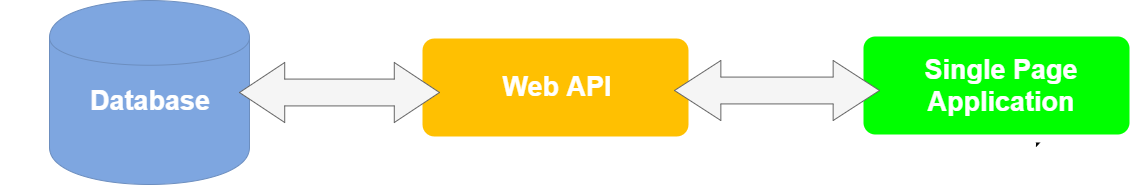
\includegraphics[height=0.15\linewidth]{introducere.png}
\centering
\caption{Arhitectura aplicației.}
\label{fig:introducere}
\end{figure}

Ideea a acestui proiect a fost inspirată de bine cunoscuta rețea de socializare \textit{Facebook} și de platforma online de jocuri \textit{Steam}.
Pe \textit{Facebook} am observat tendința oamenilor de a publica faptele bune pe care aceștia le realizează, iar pe \textit{Steam} mi-a ieșit în evidentă nevoia 
utilizatorilor de a fi premiați la orice lucru pe care îl realizează.

\textit{Facebook} este o rețea de socializare creată de către Mark Zuckerberg în anul 2004 pentru a oferi posibilitatea utilizatorilor de a contacta persoane apropiate, dar și persoane încă necunoscute.
 \textit{Facebook} este în acest moment una dintre cele mai utilizate rețele sociale din lume.
 
\textit{Steam} este o platformă distribuție digitală a jocurilor video pentru Windows, Linux și Mac dezvoltată de \textit{Valve Corporation}. 
Aceasta permite utilizatorilor să cumpere și să joace jocurile pe calculator.Această platformă de jocuri dispune totodată și de un sistem de premiere 
al utilizatorilor atât în jocuri cat și la nivel de platformă.

Considerând cele prezentate mai sus am decis realizarea undei aplicații de tip rețea de socializare ce îmbină conceptele menționate mai sus.
Astfel utilizatorii aplicației „GoodCitizen” vor beneficia de ambele necesități sociale și psihologice, mai concret sentimentele de realizare și recunoaștere/afirmare. 

